\documentclass{article}

\usepackage[heading=true]{ctex}
\usepackage[backref]{hyperref}
\usepackage{dirtree}
\usepackage{listings}
\usepackage{graphicx}
\usepackage{subfigure}
\usepackage{float}
\usepackage{filecontents}
\usepackage{geometry}
\usepackage{xcolor}
\usepackage{qtree}

\ctexset{
    section={
        number=\chinese{section},
        format+=\raggedright
    }
}
\geometry{a4paper, scale=0.7}

\title{深度学习实验三} 
\author{
1190200708 熊峰\\
\and
1190200704 管建男\\
} 
\date{\today}
\begin{document} 
\maketitle 

\newpage
\tableofcontents
\newpage

\section{环境配置}
\subsection{硬件配置}
CPU : Intel(R) Xeon(R) Silver 4214 \par
GPU : TITAN RTX 24G \par
MEM : 128G RAM  \par
\subsection{软件配置}
OS : Ubuntu 20.04.1 LTS \par
PyTorch : Stable 1.11.0  CUDA 11.3 \par
IDE : PyCharm 2021.3.2 \par


\section{模型结构}
\subsection{VGG}

\begin{figure}[H]
    \begin{center}
        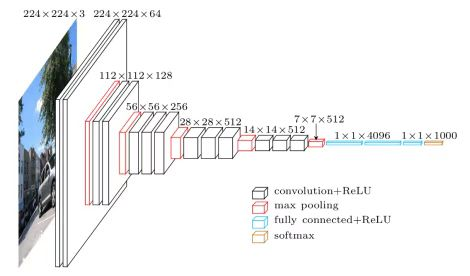
\includegraphics[width=12cm]{figures/VGG16Model.jpg}
        \caption{VGG16 Model}
        \label{fig:1}
    \end{center}
\end{figure}
\par
本部分主要实现了VGG16模型\cite{simonyan2014very}。\par 
第一部分经过两层卷积(在所有卷积操作后加上ReLU),此时输出为64*224*224.\par
第二部分经过一层池化层,再通过两层卷积层,此时输出为256*56*56.\par
第三部分经过一层池化层,再通过三层卷积层,此时输出为512*14*14.\par
第四部分经过一层池化层,此时输出为512*7*7.\par 
第五部分主要为全连接层,将上一部分输出映射为12维的向量。\par


\subsection{ResNet}

深的神经网络难以训练,何恺明提出残差学习\cite{he2016deep}的框架,使训练非常深的网络比之前容易很多。其将各层重新表述为学习参考层输入的残差函数。\par 

当网络很深时,容易出现梯度消失、梯度爆炸等问题,通常采用初始化的权重和在中间加入Normalization,例如BN等,可以校验每个层之间的输出和他的梯度的均值和方差。
使用上述方法可以使网络收敛,这时一个次要的问题就暴露出来了。随着网络的深度增加,准确度会达到饱和,然后迅速退化,这种退化并不是由于过拟合引起的,而在一个适当的深度模型上增加更多的层会导致更高的训练误差。\par

因此ResNet中提出了残差学习框架,其不希望几个堆积层直接训练所需的映射,而是让这些层训练一个残差的映射$\mathcal{F}(x)=\mathcal{H}(x)-x$。
\begin{figure}[H]
    \begin{center}
        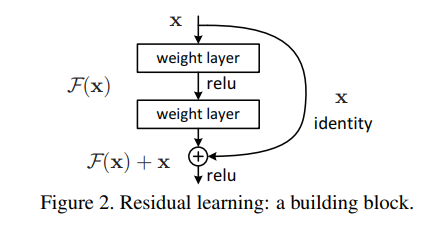
\includegraphics[width=12cm]{figures/ResNetBlock.png}
        \caption{ResNet Block}
        \label{fig:2}
    \end{center}
\end{figure}
\par

x为浅层网络学习到表征,经过堆叠的层后得到的映射为$\mathcal{H}(x)$,但不让这个堆叠的网络直接训练得到$\mathcal{H}(x)$,因为直接学习到的很有可能效果不如浅层网络,因此希望它学习$\mathcal{F}(x)=\mathcal{H}(x)-x$,这个函数更易于优化,假定此时恒等映射更好,即$\mathcal{H}(x)=x$,那么可以使堆叠的网络学习到的为$\mathcal{F}(x){\rightarrow}0$,即将残差部分推到0,此时$\mathcal{H}(x)=x$,此时至少可以保证效果不低于浅层网络,若堆叠的层获得了更好的表征,很有可能提升网络的性能。

\subsection{SENet}

SENet\cite{hu2018squeeze}是ImageNet 2017的冠军模型,其主要思想为,对于每个输出channel,预测一个常数权重,对每个channel加权。其可以很方便地集成到现有网络中,提升网络性能,并且代价很小。

\begin{figure}[H]
    \centering
    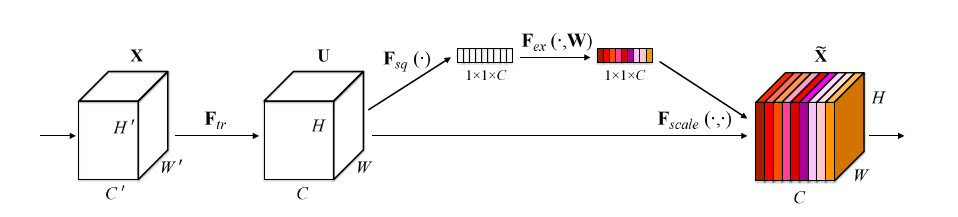
\includegraphics[width=0.8\textwidth]{figures/senet.png}
    \caption{SENet}
\end{figure}

如图为,SENet和ResNet的结合,第一层的FC会把通道降下来,然后第二层FC再把通道升上去,得到和通道数相同的C个权重,每个权重用于给对应的一个通道进行加权。上图中的r就是缩减系数,实验确定选取16,可以得到较好的性能并且计算量相对较小。

\begin{figure}[H]
    \centering
    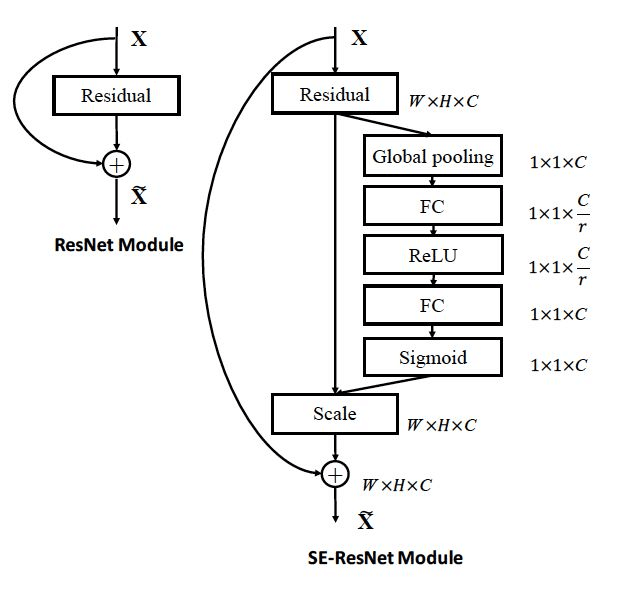
\includegraphics[width=0.7\textwidth]{figures/senetwithresnet.png}
    \caption{SENet和ResNet的结合}
\end{figure}


\section{优化方法}
\subsection{公共优化部分}
\subsubsection{优化器}
Adam: 使用Adam训练效果较好,在较多模型都得到比较好的结果。\par 
SGD: 使用SGD训练时,大多数模型效果很差,Micro F1 Score维持在0.1-0.2.\par


\subsubsection{数据增强}
进行data augmentation(翻转、旋转、移位等操作)对比。



\subsection{其他优化方法}

引入新的模块/换用更好的模型等
内容不限,可有效提升性能即可

增加一种Swin Transformer模型\cite{liu2021swin}。

使用K折交叉验证。


\section{训练过程}

\subsection{无数据增强的情况}

VGG训练过程中的micro F1和macro F1如图\ref{VGG-f1s}

\begin{figure}[H]
    \begin{minipage}[H]{0.5\linewidth}
        \centering
        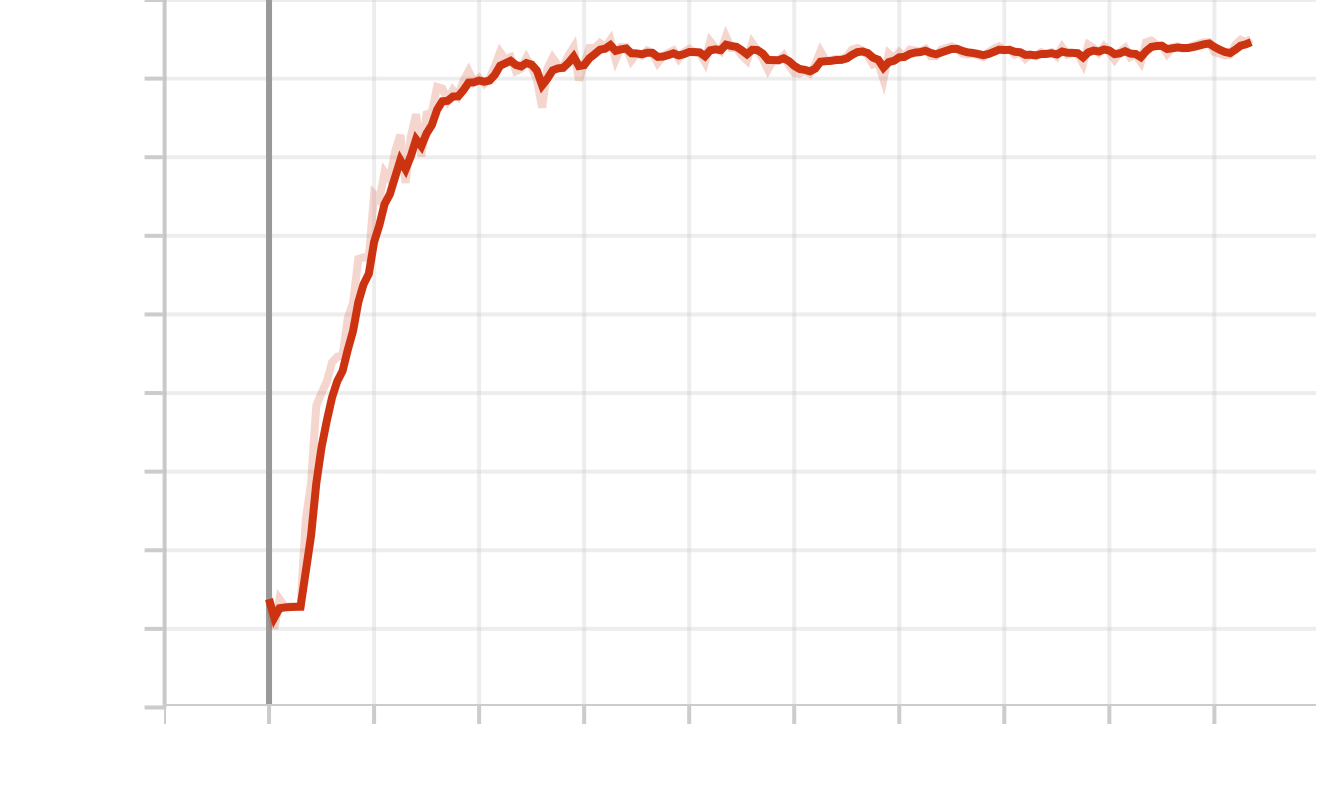
\includegraphics[width=\textwidth]{figures/vgg_noaug_microf1score_dev.png}
    \end{minipage}
    \begin{minipage}[H]{0.5\linewidth}
        \centering
        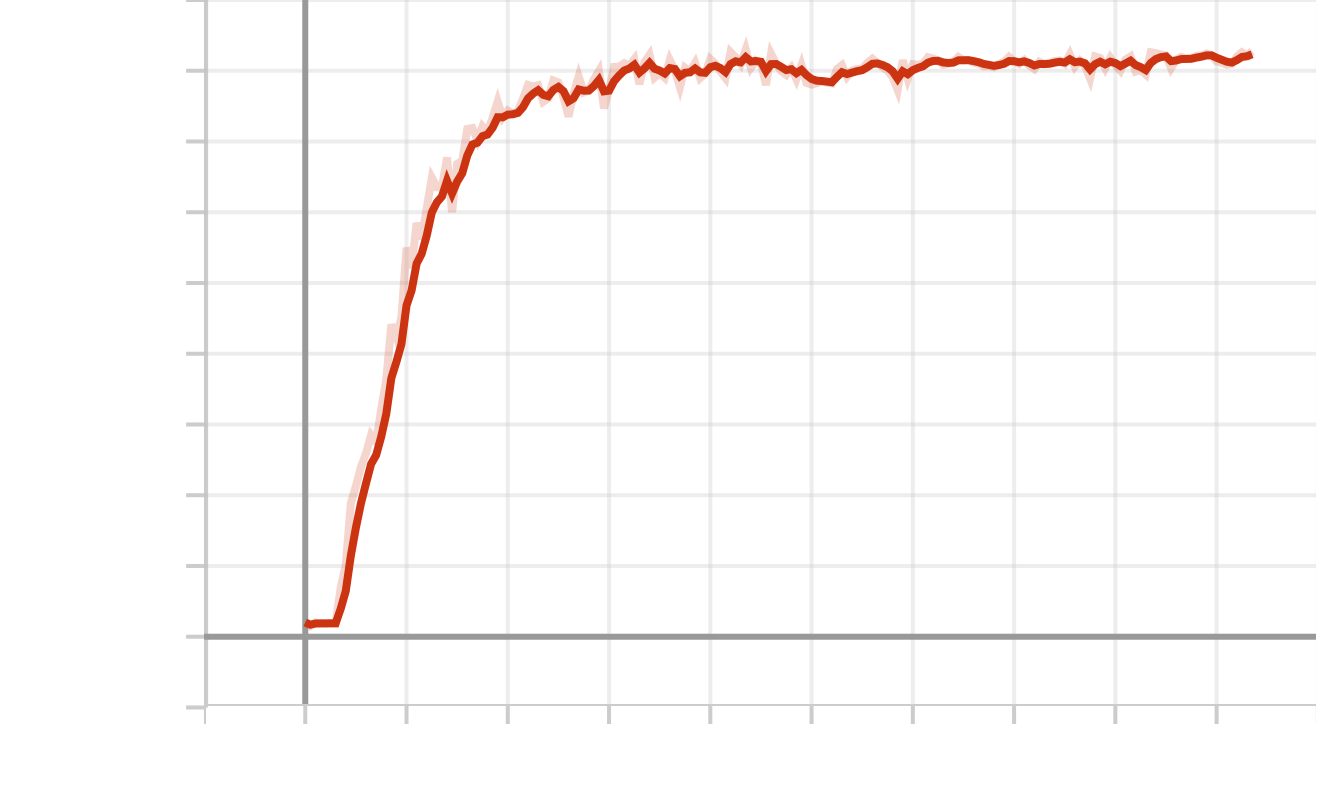
\includegraphics[width=\textwidth]{figures/vgg_noaug_macrof1score_dev.png}
    \end{minipage}
    \caption{VGG训练过程中的micro F1和macro F1}
    \label{VGG-f1s}
\end{figure}

ResNet训练过程中的micro F1和macro F1如图\ref{ResNet-f1s}

\begin{figure}[H]
    \begin{minipage}[H]{0.5\linewidth}
        \centering
        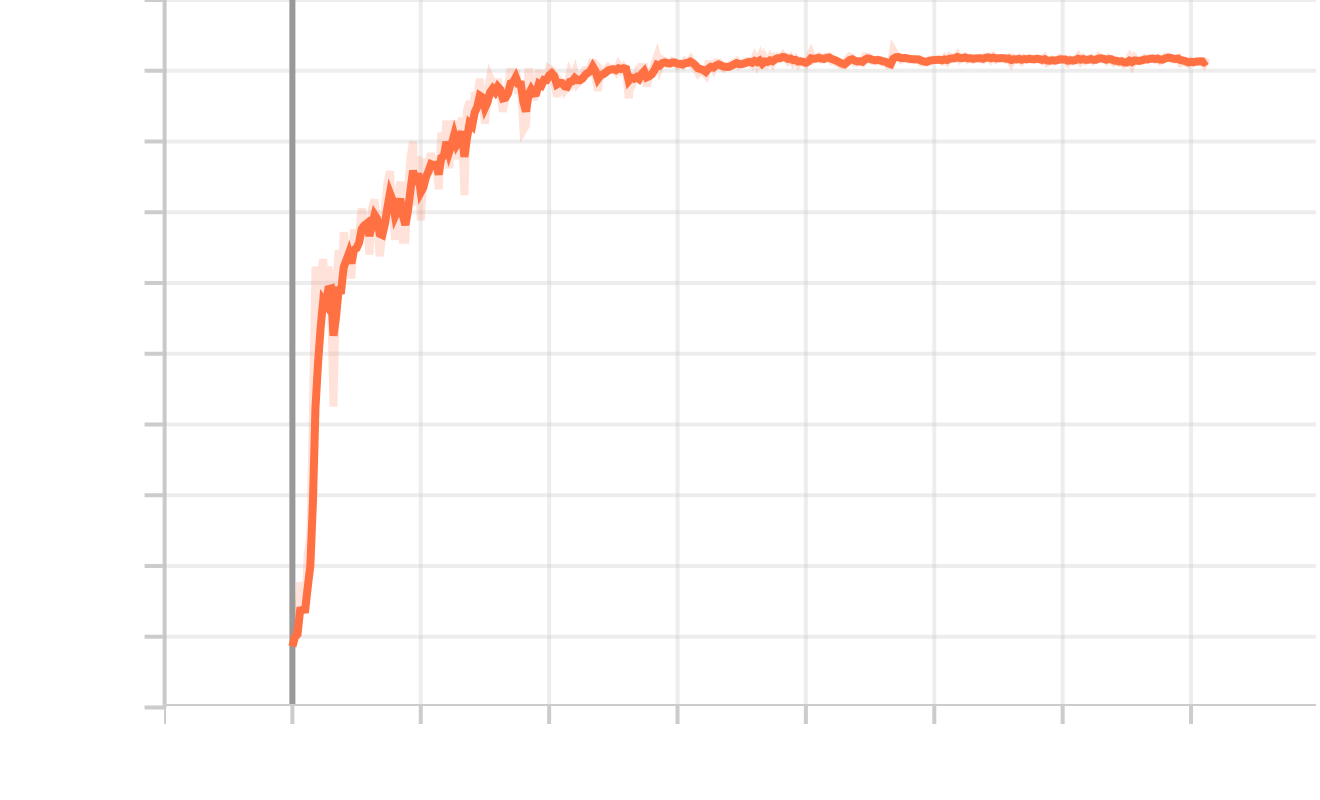
\includegraphics[width=\textwidth]{figures/resnet_noaug_microf1score_dev.png}
    \end{minipage}
    \begin{minipage}[H]{0.5\linewidth}
        \centering
        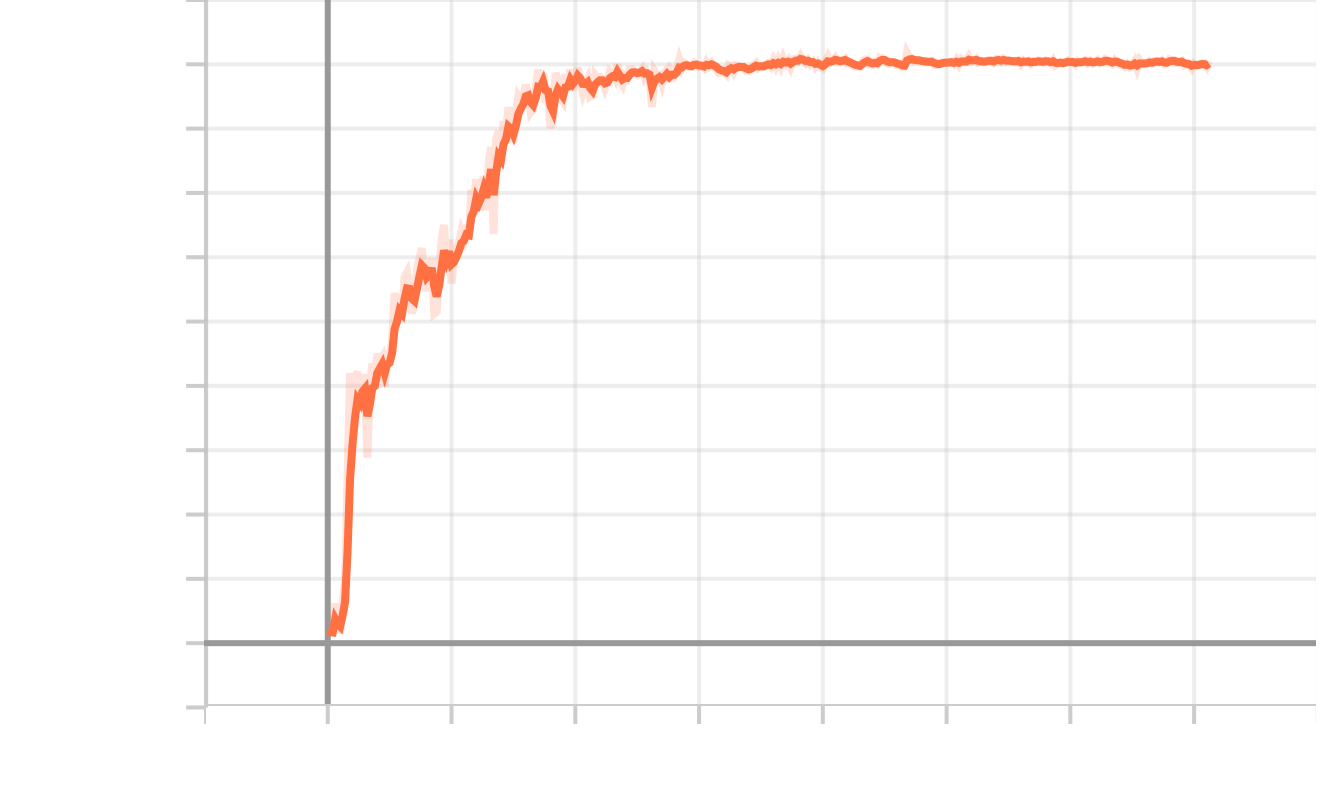
\includegraphics[width=\textwidth]{figures/resnet_noaug_macrof1score_dev.png}
    \end{minipage}
    \caption{ResNet训练过程中的micro F1和macro F1}
    \label{ResNet-f1s}
\end{figure}

SENet训练过程中的micro F1和macro F1如图\ref{SENet-f1s}

\begin{figure}[H]
    \begin{minipage}[H]{0.5\linewidth}
        \centering
        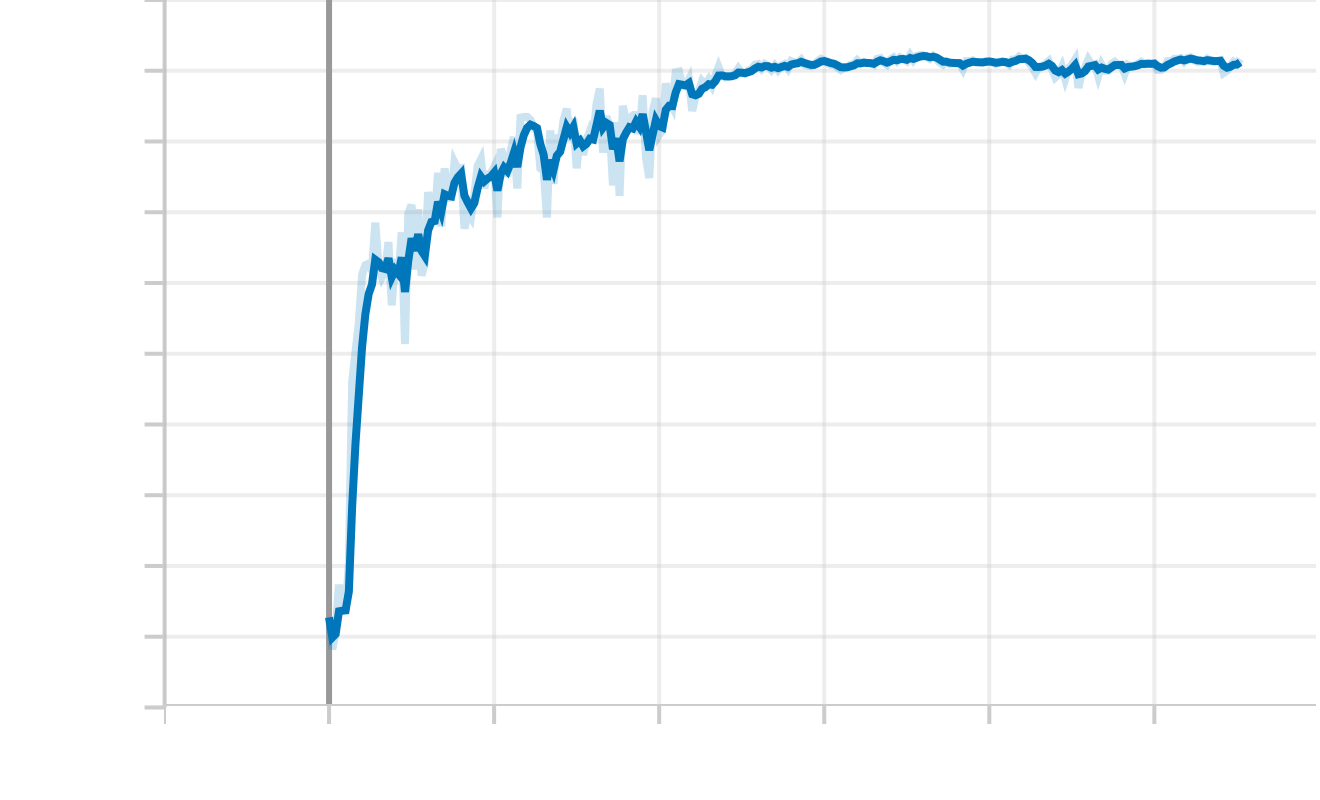
\includegraphics[width=\textwidth]{figures/senet_noaug_microf1score_dev.png}
    \end{minipage}
    \begin{minipage}[H]{0.5\linewidth}
        \centering
        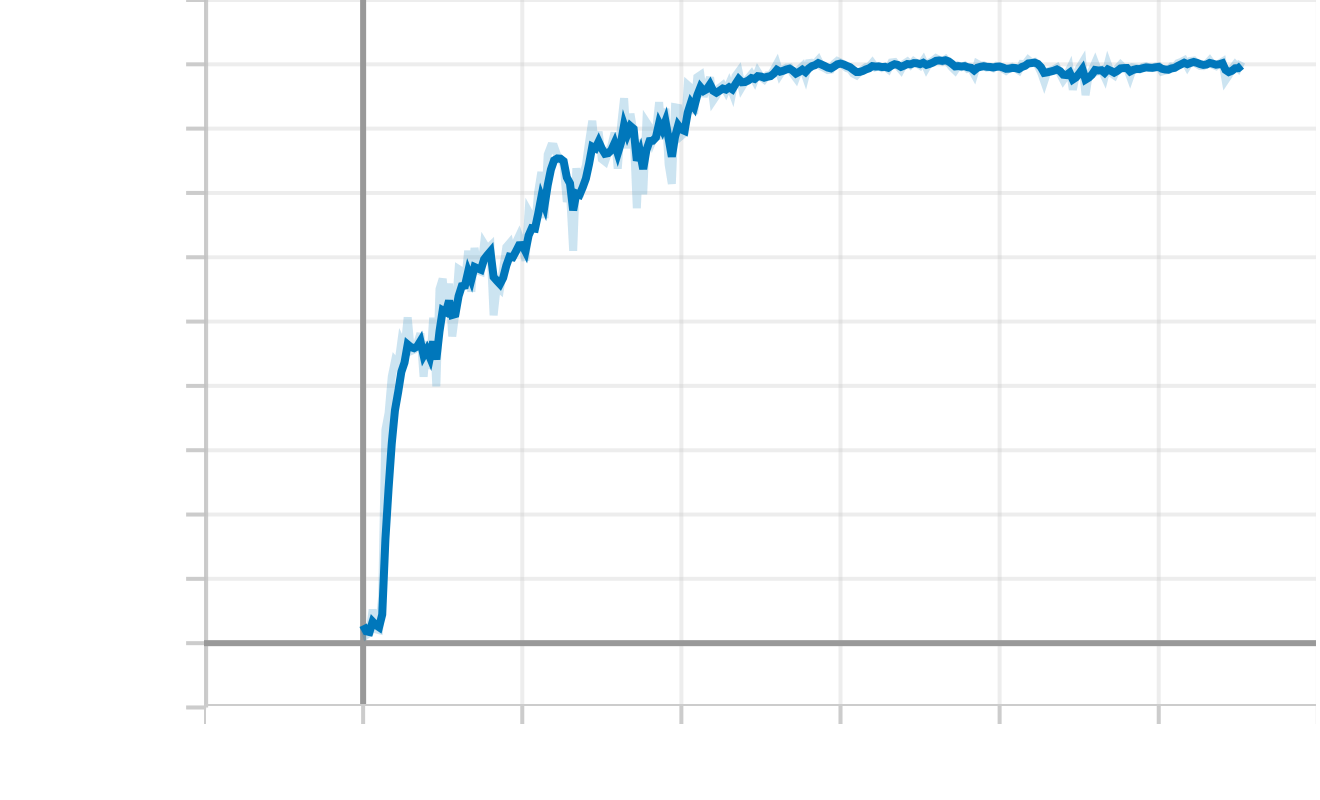
\includegraphics[width=\textwidth]{figures/senet_noaug_macrof1score_dev.png}
    \end{minipage}
    \caption{SENet训练过程中的micro F1和macro F1}
    \label{SENet-f1s}
\end{figure}

\subsection{有数据增强的情况}

采用的数据增强包括旋转(rot)、翻转(flp)、色彩增强,
其中色彩增强又包括分色(pst)和曝光(slr)。
数据增强的具体操作方式为:
在原始数据集的基础上,通过水平翻转(hflp)和垂直翻转(vflp)产生四份新的数据集,
再对每一份数据集做色彩增强。

采用了全部的数据增强方式,VGG训练过程中的micro F1和macro F1如图\ref{VGG-f1s-aug}

\begin{figure}[H]
    \begin{minipage}[H]{0.5\linewidth}
        \centering
        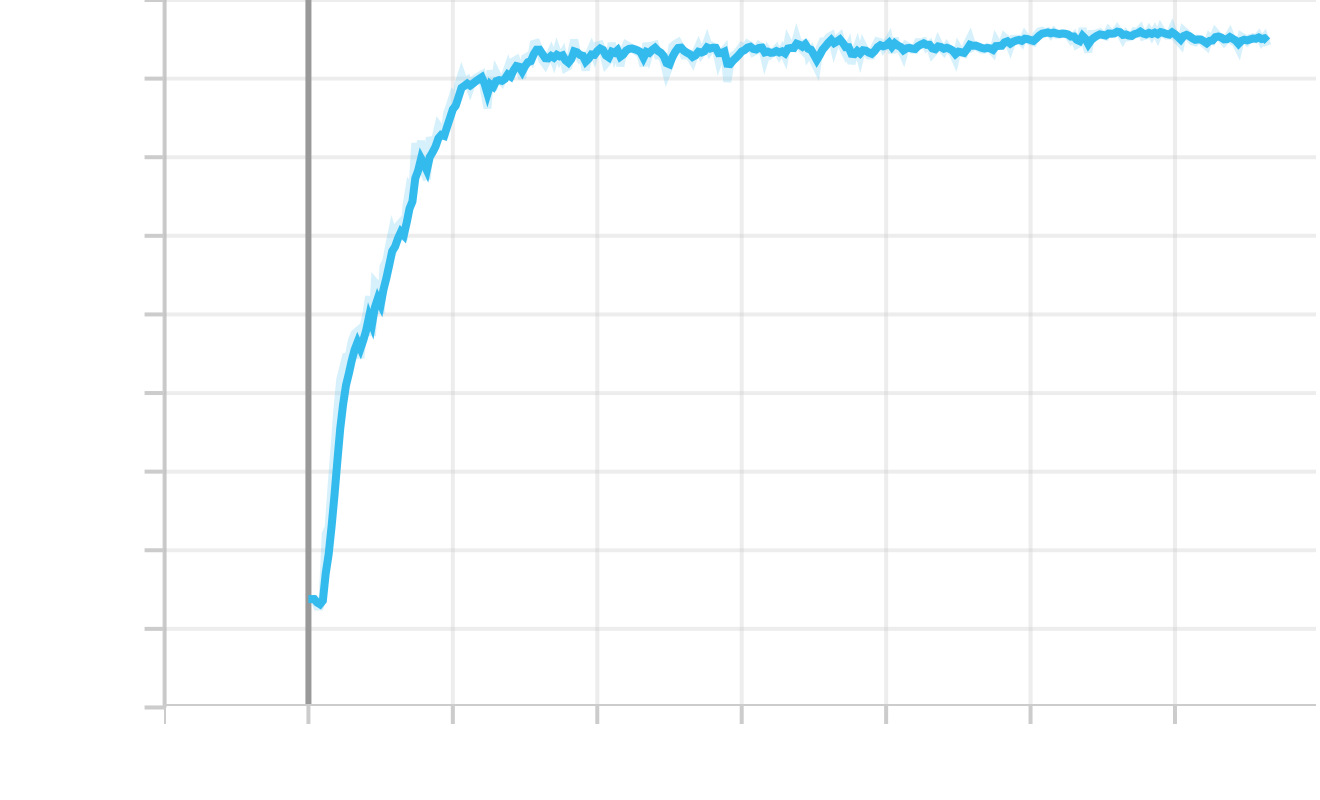
\includegraphics[width=\textwidth]{figures/vgg_aug_microf1score_dev.png}
    \end{minipage}
    \begin{minipage}[H]{0.5\linewidth}
        \centering
        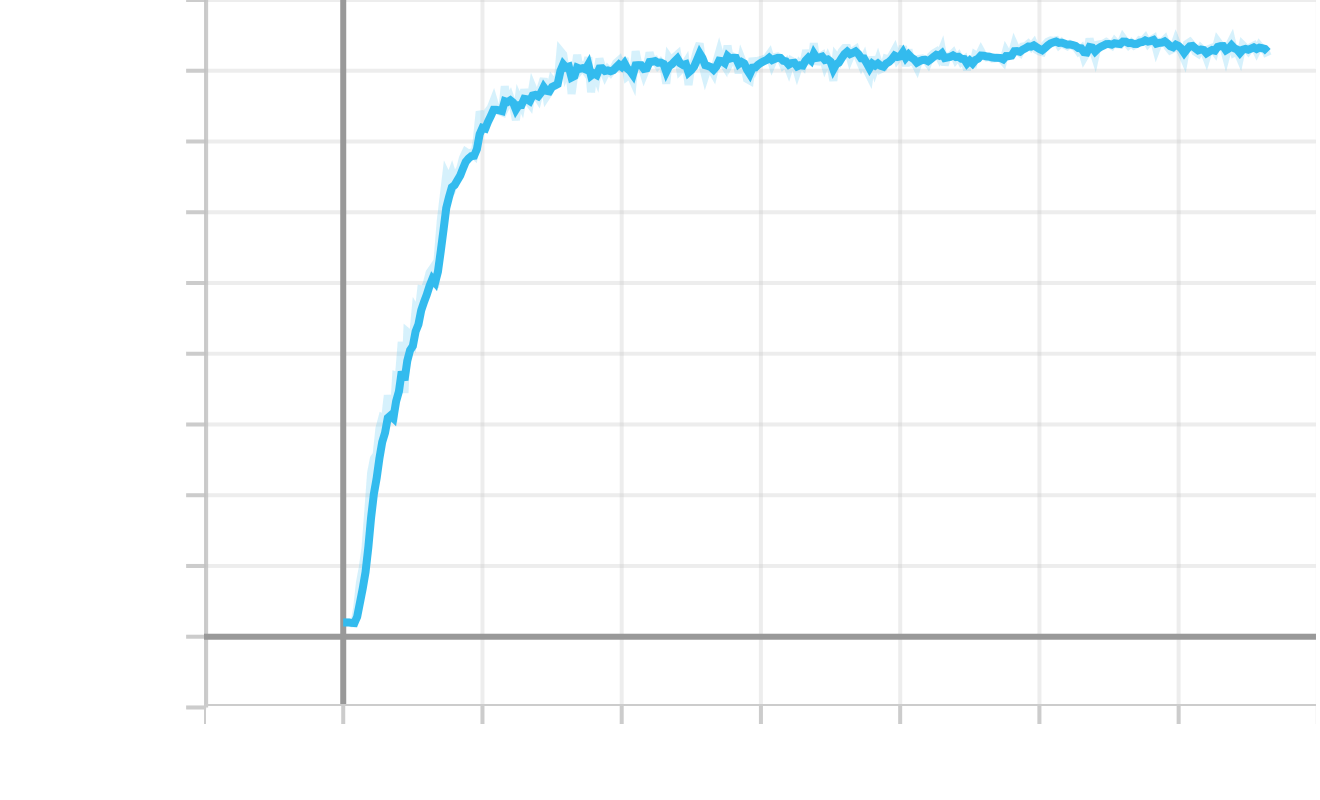
\includegraphics[width=\textwidth]{figures/vgg_aug_macrof1score_dev.png}
    \end{minipage}
    \caption{采用了全部的数据增强方式,VGG训练过程中的micro F1和macro F1}
    \label{VGG-f1s-aug}
\end{figure}

采用了全部的数据增强方式,ResNet训练过程中的micro F1和macro F1如图\ref{ResNet-f1s-aug}

\begin{figure}[H]
    \begin{minipage}[H]{0.5\linewidth}
        \centering
        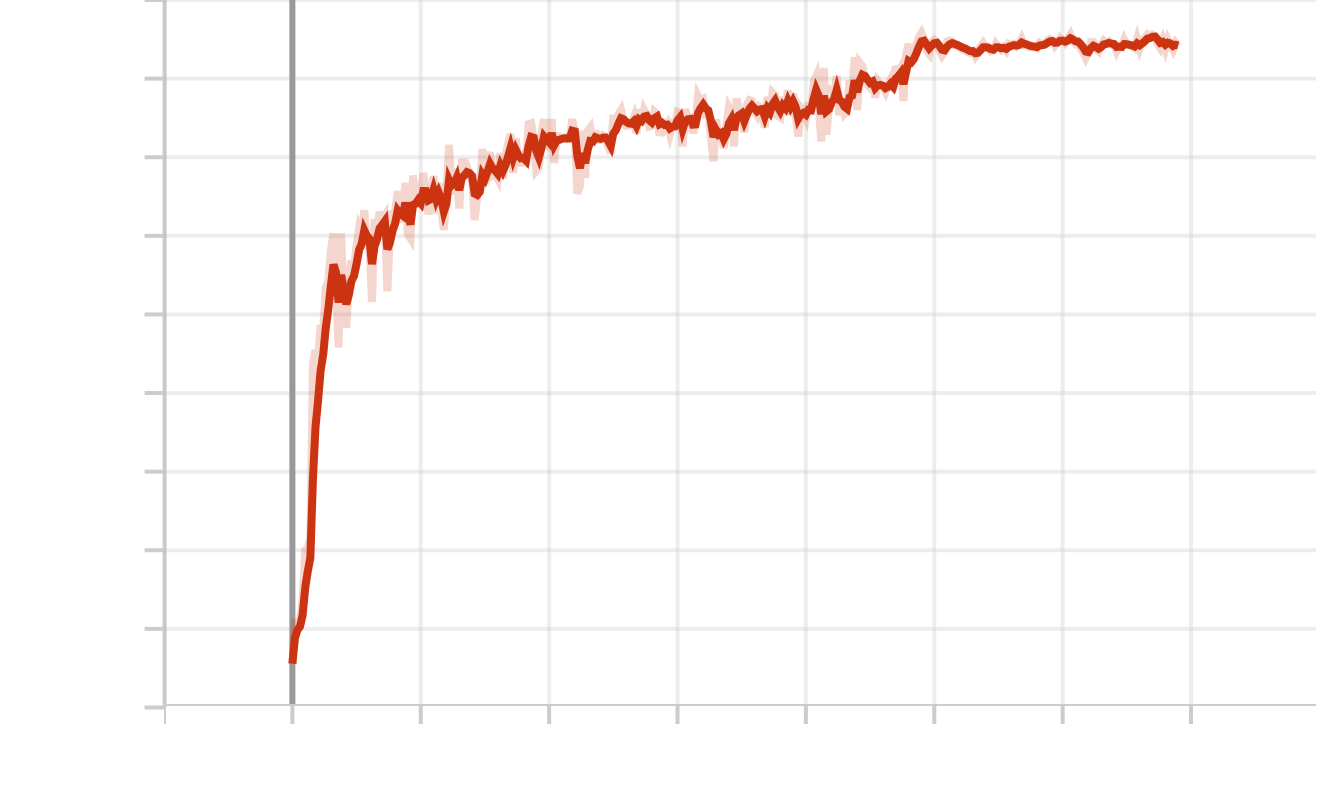
\includegraphics[width=\textwidth]{figures/resnet_aug_microf1score_dev.png}
    \end{minipage}
    \begin{minipage}[H]{0.5\linewidth}
        \centering
        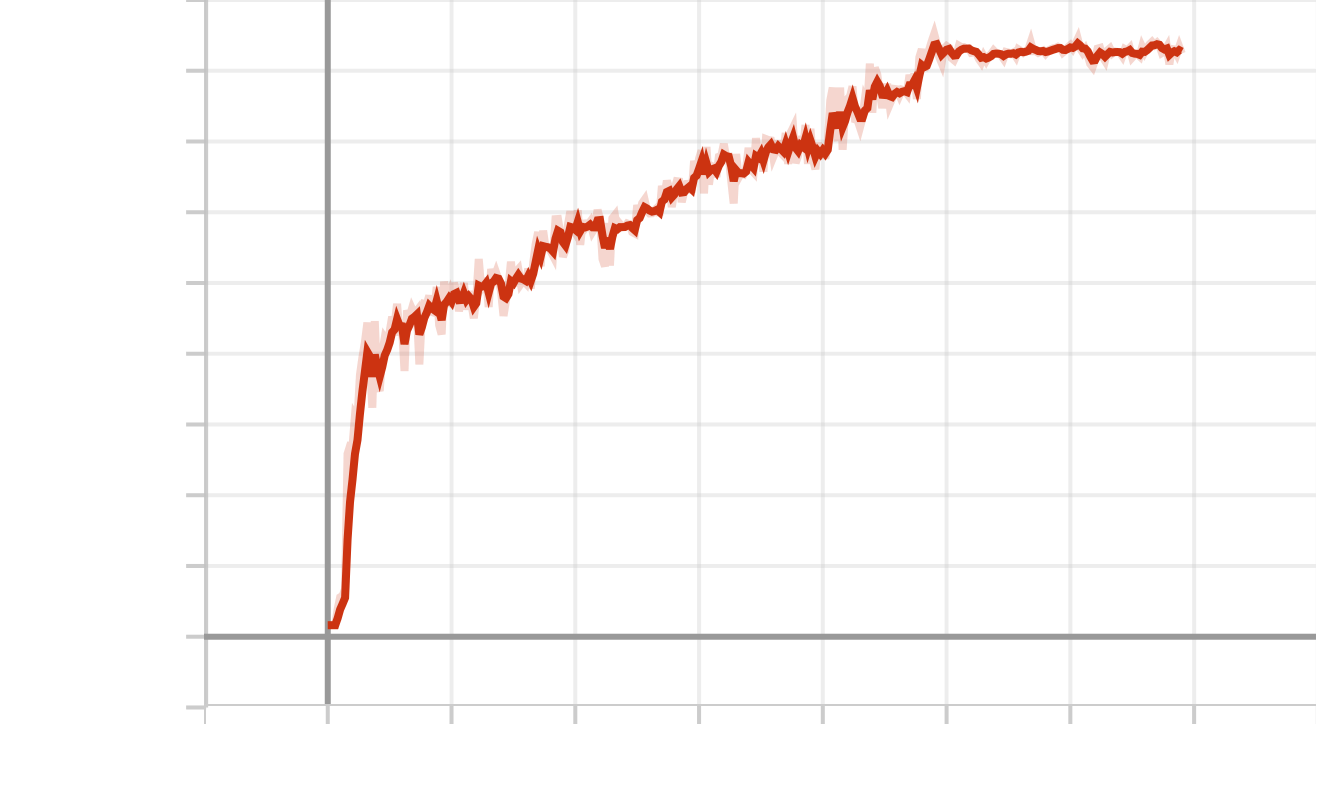
\includegraphics[width=\textwidth]{figures/resnet_aug_macrof1score_dev.png}
    \end{minipage}
    \caption{采用了全部的数据增强方式,ResNet训练过程中的micro F1和macro F1}
    \label{ResNet-f1s-aug}
\end{figure}

采用了全部的数据增强方式,SENet训练过程中的micro F1和macro F1如图\ref{SENet-f1s-aug}

\begin{figure}[H]
    \begin{minipage}[H]{0.5\linewidth}
        \centering
        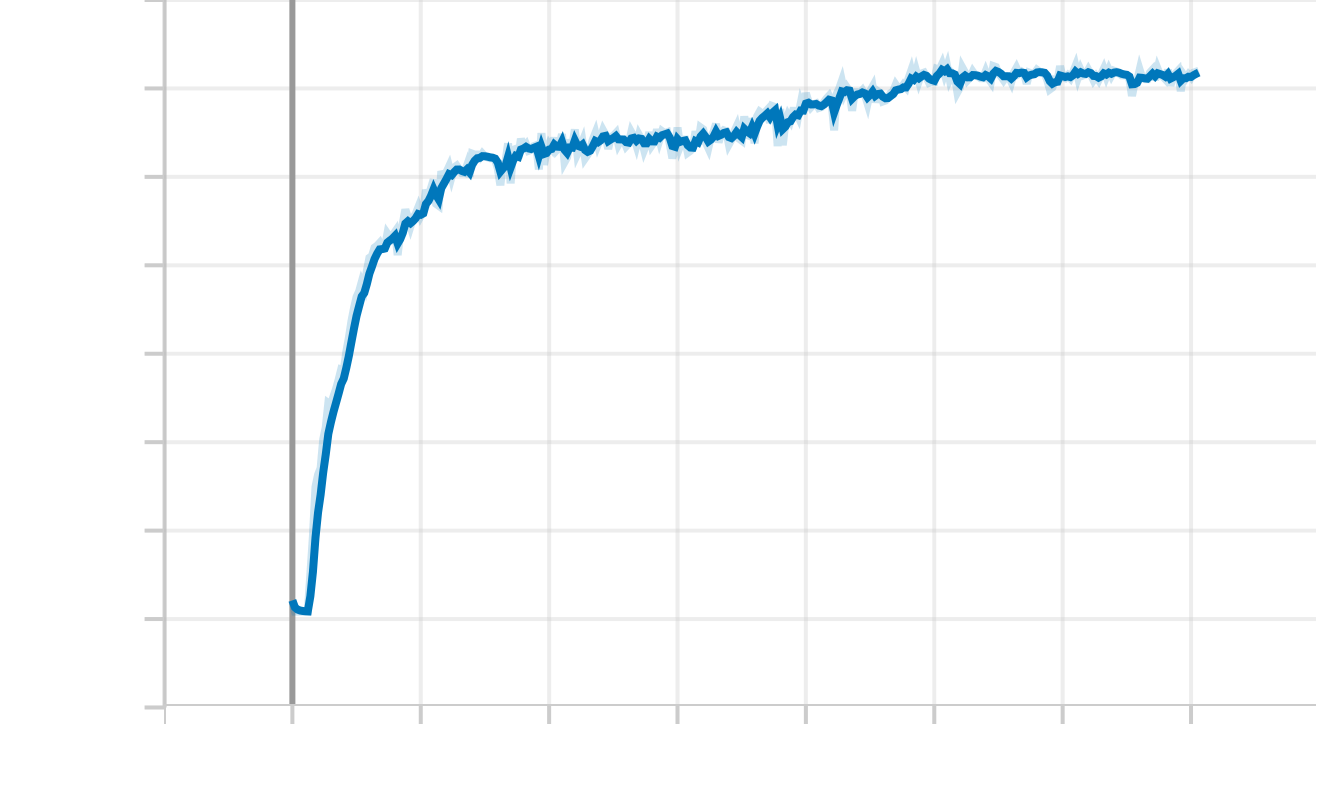
\includegraphics[width=\textwidth]{figures/senet_aug_microf1score_dev.png}
    \end{minipage}
    \begin{minipage}[H]{0.5\linewidth}
        \centering
        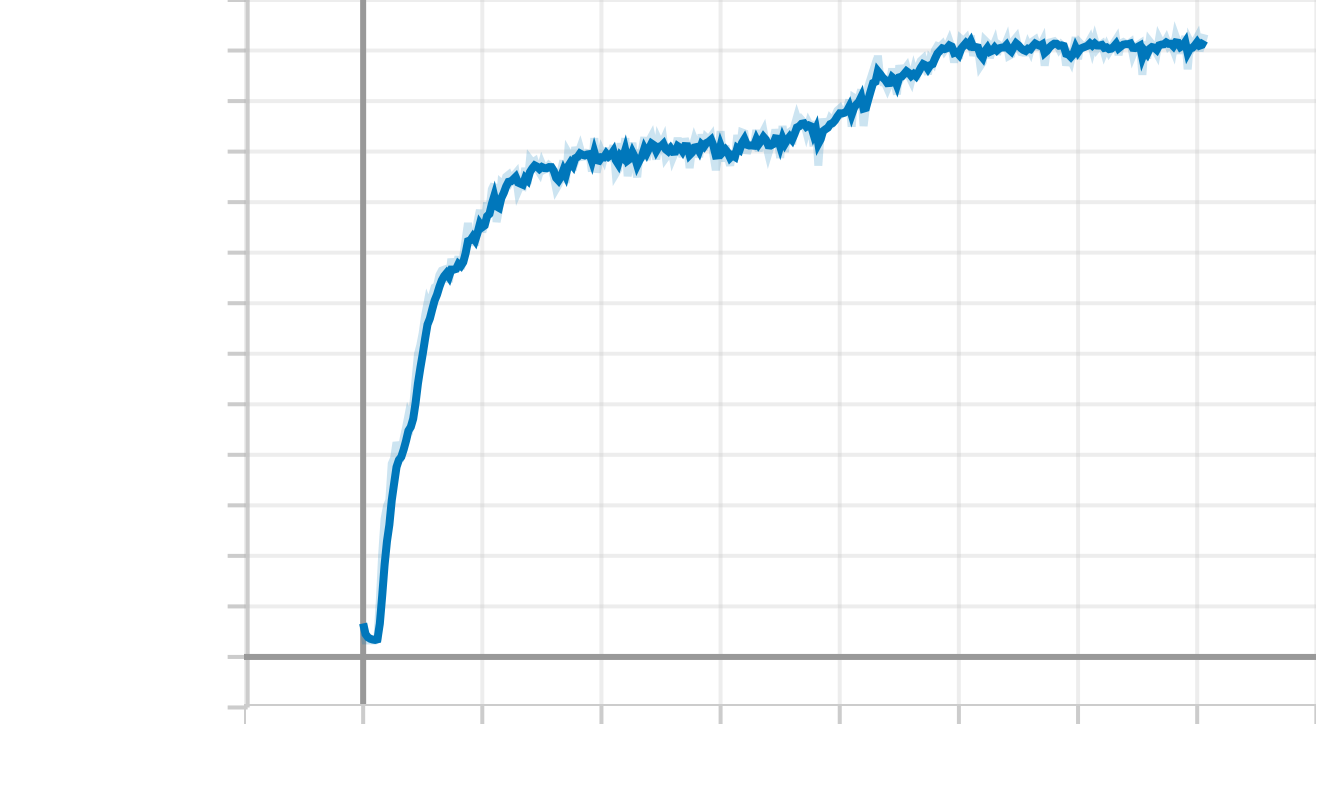
\includegraphics[width=\textwidth]{figures/senet_aug_macrof1score_dev.png}
    \end{minipage}
    \caption{采用了全部的数据增强方式,SENet训练过程中的micro F1和macro F1}
    \label{SENet-f1s-aug}
\end{figure}

\subsection{进一步增强:使用K折交叉验证的Swin Transformer模型}

使用K折交叉验证的Swin Transformer,
训练过程中的micro F1和macro F1如图\ref{swintrans-f1s}
由于实验中K取值为5,因此下图中展示了这5个模型的结果。

\begin{figure}[H]
    \begin{minipage}[H]{0.5\linewidth}
        \centering
        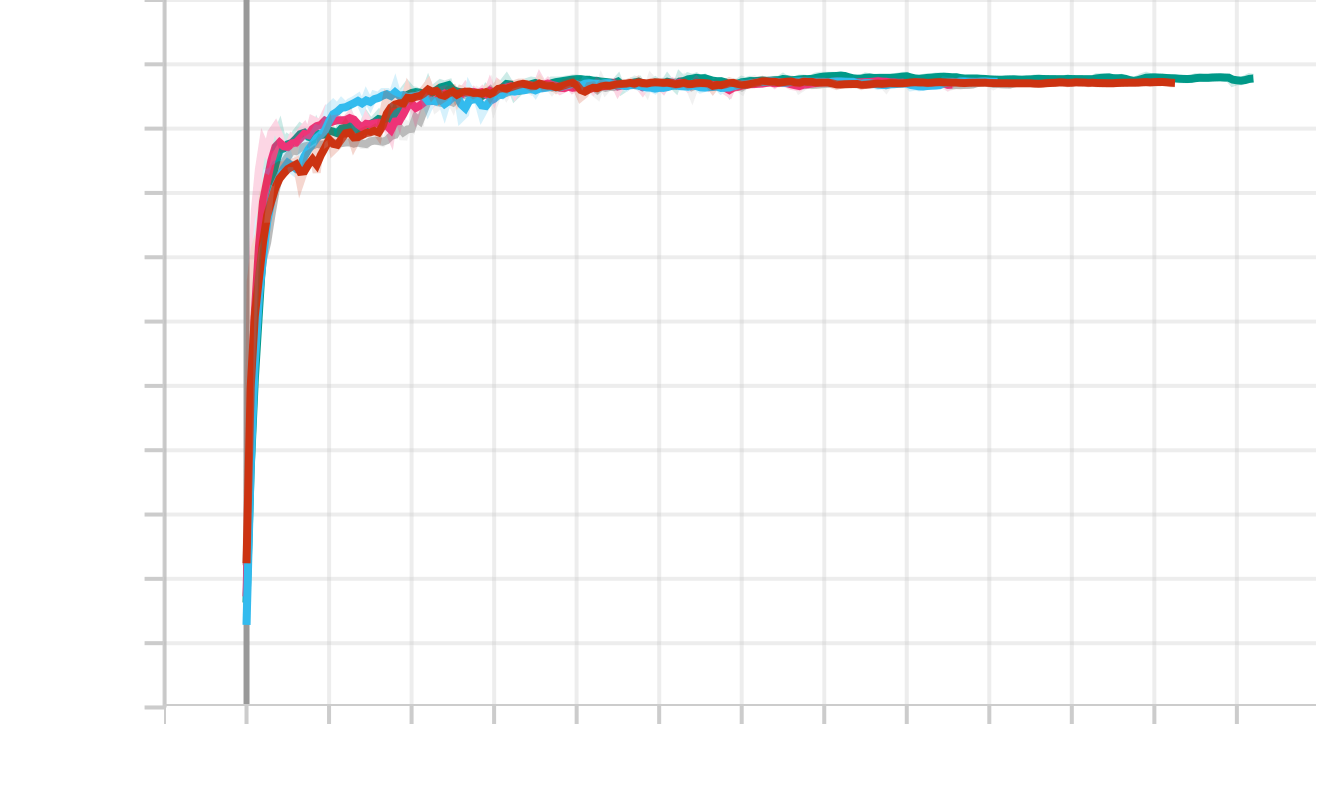
\includegraphics[width=\textwidth]{figures/swintrans_noaug_microf1score_dev.png}
    \end{minipage}
    \begin{minipage}[H]{0.5\linewidth}
        \centering
        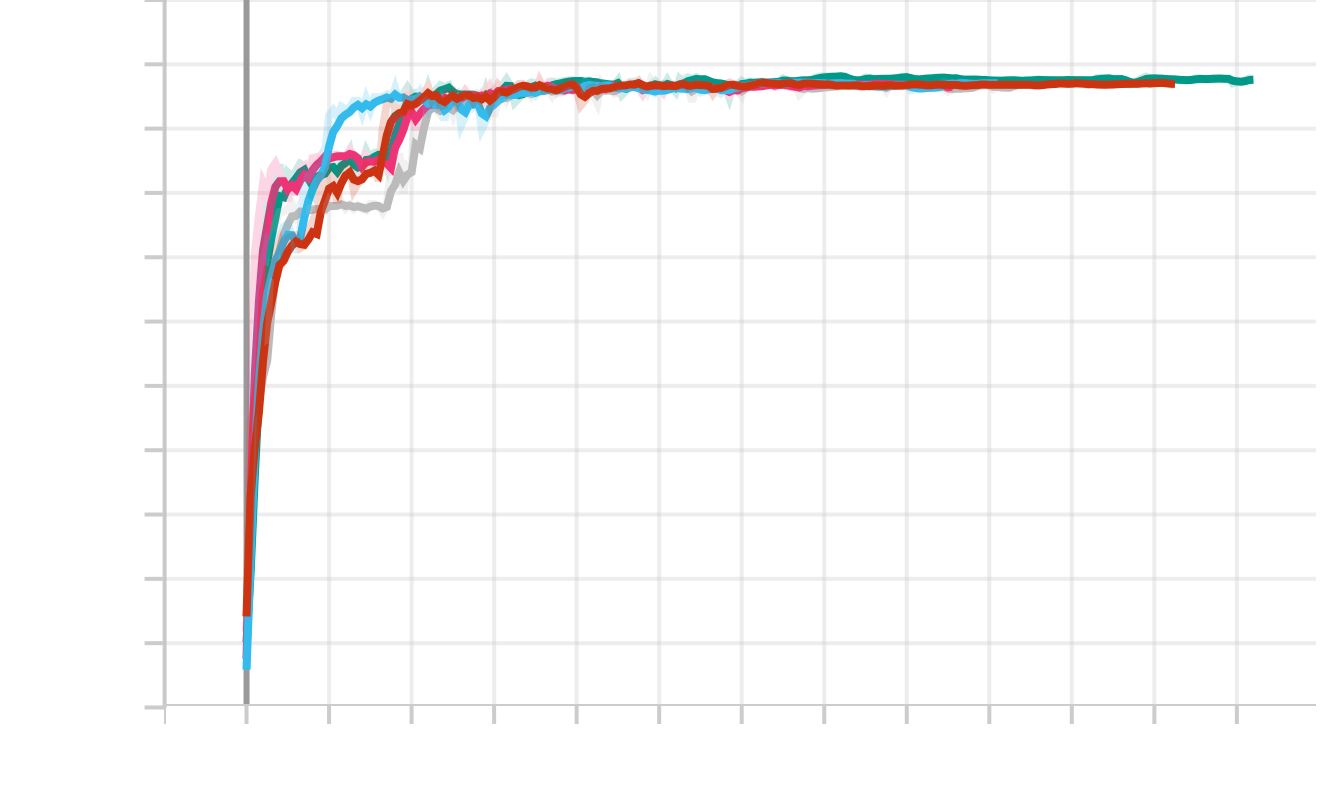
\includegraphics[width=\textwidth]{figures/swintrans_noaug_macrof1score_dev.png}
    \end{minipage}
    \caption{Swin Transformer训练过程中的micro F1和macro F1}
    \label{swintrans-f1s}
\end{figure}

\section{实验结果}

各个模型实验结果如图\ref{all_models_cmp}

\begin{table}[H]
    \centering
    \begin{tabular}{lllll}
        \hline
        \textbf{Model}   & \textbf{Augmentation}     & \textbf{Micro F1} & \textbf{Macro F1} & \textbf{Kaggle} \\
        \hline
        \hline
        VGG16            & None                      & 85.05\%           & 82.76\%           & 85.39\%         \\
        VGG16            & vflp+hflp+pst+slr         & 84.21\%           & 82.08\%           & 85.77\%         \\
        ResNet18         & None                      & 92.84\%           & 91.76\%           & 92.19\%         \\
        ResNet18         & vflp+hflp+pst+slr         & 82.44\%           & 82.44\%           & 85.89\%         \\
        SENet18          & None                      & 92.21\%           & 90.96\%           & 91.94\%         \\
        SENet18          & vflp+hflp+pst+slr         & 72.74\%           & 61.61\%           & 62.97\%         \\
        Swin Transformer & feature extractor + Kfold & 97.28\%           & 97.06\%           & 97.48\%         \\
        \hline
    \end{tabular}
    \label{all_models_cmp}
    \caption{各个模型实验结果}
\end{table}

\section{成员分工}
\subsection{熊峰}
\begin{enumerate} 
    \item 实现VGG、ResNet、SENet等模型,个人优化使用Swin Transformer模型。
    \item 编写训练过程
          \begin{itemize}
              \item 编写基础训练过程
              \item 个人优化:训练过程增加K折交叉验证
          \end{itemize}
    \item 训练SENet、更新模型使用Swin Transformer模型
    \item 撰写报告模型部分
\end{enumerate}
\subsection{管健男}
\begin{enumerate} 
    \item 实现 argparser模块
    \item 实现支持K折交叉验证的数据加载器
    \item 实现数据增强模块
    \item 训练 VGG、ResNet模型
    \item 撰写报告训练结果部分
\end{enumerate}


\bibliographystyle{unsrt}
\bibliography{refs}
\end{document}
